\documentclass[,]{sagej}

\usepackage{moreverb,url,natbib, multirow, tabularx}
\usepackage[colorlinks,bookmarksopen,bookmarksnumbered,citecolor=red,urlcolor=red]{hyperref}



% tightlist command for lists without linebreak
\providecommand{\tightlist}{%
  \setlength{\itemsep}{0pt}\setlength{\parskip}{0pt}}

% From pandoc table feature
\usepackage{longtable,booktabs,array}
\usepackage{calc} % for calculating minipage widths
% Correct order of tables after \paragraph or \subparagraph
\usepackage{etoolbox}
\makeatletter
\patchcmd\longtable{\par}{\if@noskipsec\mbox{}\fi\par}{}{}
\makeatother
% Allow footnotes in longtable head/foot
\IfFileExists{footnotehyper.sty}{\usepackage{footnotehyper}}{\usepackage{footnote}}
\makesavenoteenv{longtable}


\usepackage{booktabs}


\begin{document}


\setcitestyle{aysep={,}}

\title{A Proposed Data Standard for Municipal Zoning Regulations}

\runninghead{}

\author{Carole Turley Voulgaris\affilnum{}, Paul Salama\affilnum{}, Luke Reeve\affilnum{}, Elizabeth Christoforetti\affilnum{}}

\affiliation{\affilnum{}{}\\\affilnum{}{}}



\begin{abstract}
About 200 words. Unclear about if there is a limit
\end{abstract}

\keywords{ZoningOpen data}

\maketitle

Introductory text

\hypertarget{literature-review}{%
\section{Literature review}\label{literature-review}}

Introduce the literature review

\hypertarget{prior-and-current-efforts-to-digitize-zoning-data}{%
\subsection{Prior and current efforts to digitize zoning data}\label{prior-and-current-efforts-to-digitize-zoning-data}}

Describe the National Zoning Atlas and affiliated teams, MAPC data, the Georgia Tech
effort. Others?

\hypertarget{other-open-data-standards-for-local-government}{%
\subsection{Other open data standards for local government}\label{other-open-data-standards-for-local-government}}

Describe GTFS, GBFS, MDS, OpenStreetMap others? Are there any examples not in mobility?

\hypertarget{method}{%
\section{Method}\label{method}}

This section describes the zoning standard and the analysis method. This may
be the bulk of the paper.

\hypertarget{zoning-standard}{%
\subsection{Zoning standard}\label{zoning-standard}}

Describe the zoning standard

\hypertarget{core-constraints}{%
\subsubsection{Core constraints}\label{core-constraints}}

OZFS begins with a set of core constraints: components that are necessary to
establish the maximum allowable bulking or building envelope on any lot. Our
work-in-progress list of these constraints are captured within an Airtable
titled \href{https://airtable.com/invite/l?inviteId=invIE9Rq8BJxoRZe9\&inviteToken=c24d20d82c00f933e02ca4d7f9b78088b2eaefcef049f3691df85eb48f858fbc\&utm_medium=email\&utm_source=product_team\&utm_content=transactional-alerts}{OZFS schema}. (NOTE: Do I need to create an account to access this???)

Each constraint is categorized into a core component of what is known as bulking, which is the process through which structures take their form on a lot within the modern-day zoning concept (the bucket is titled ``core bulking component''). OpenZoning considers these components to be the core devices through which modern society has used zoning to conceptualize and abstract the tangible resource of land as discrete containers for bulks, i.e.~structures and buildings. These containers are called lots -- discrete areas of land plus the volumes of air above and earth beneath them -- and are the base units of zoning. When applied to the lot, modern society's conceptualization of land is executed through a set of components meant to control the realization of bulks (i.e.~bulking) on these lots. They are:

\begin{itemize}
\tightlist
\item
  buildable area limits
\item
  height limits
\item
  structure envelopes
\item
  number of structures
\item
  types of structures
\item
  relationship between structures
\item
  number of units limits
\item
  types of floor use
\end{itemize}

This list is a work in progress, and correctly identifying these components is essential to OpenZoning's goal of creating a standard machine-readable format that can accomodate the wide swathe of zoning codes that exist across America, and across the world.

\hypertarget{analysis-of-accessory-dwelling-unit-capacity}{%
\subsection{Analysis of accessory dwelling unit capacity}\label{analysis-of-accessory-dwelling-unit-capacity}}

Describe both a naive approach that would be the best you can do with other methods
and the approach we could take with this data.

\hypertarget{naive-approach}{%
\subsubsection{Naive approach}\label{naive-approach}}

Best you could do with a spreadsheet

\hypertarget{proposed-approach}{%
\subsubsection{Proposed approach}\label{proposed-approach}}

Figures and tables \emph{with captions} can also be cross-referenced from elsewhere in your book using \texttt{\textbackslash{}@ref(fig:chunk-label)} and \texttt{\textbackslash{}@ref(tab:chunk-label)}, respectively.

See Figure \ref{fig:nice-fig}.

\begin{verbatim}
par(mar = c(4, 4, .1, .1))
plot(pressure, type = 'b', pch = 19)
\end{verbatim}

\begin{figure}

{\centering 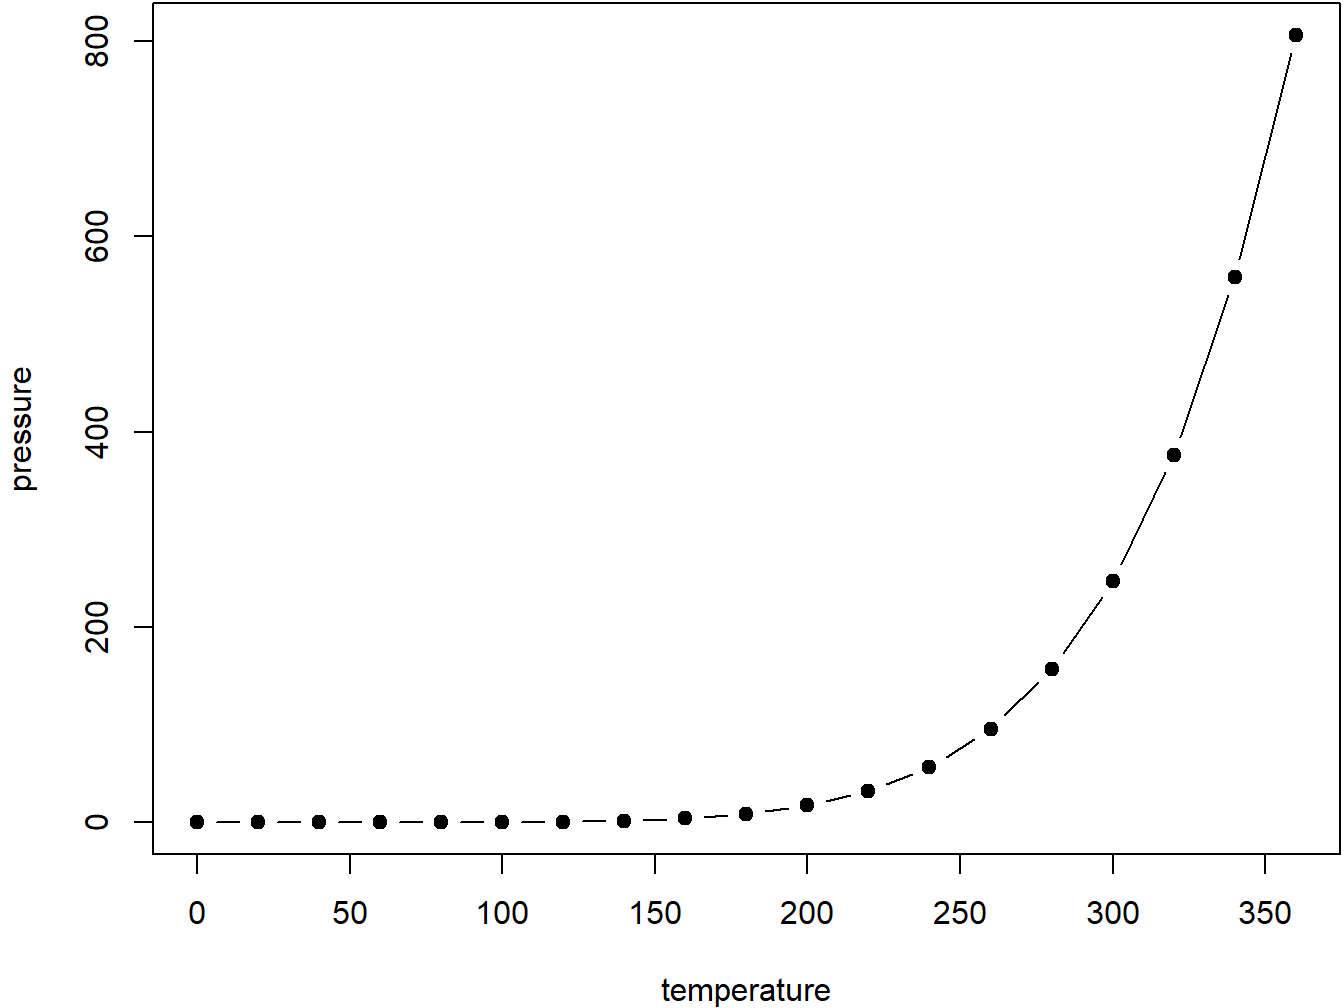
\includegraphics[width=0.8\linewidth]{_main_files/figure-latex/nice-fig-1} 

}

\caption{Here is a nice figure!}\label{fig:nice-fig}
\end{figure}

Don't miss Table \ref{tab:nice-tab}.

\begin{verbatim}
knitr::kable(
  head(pressure, 10), caption = 'Here is a nice table!',
  booktabs = TRUE
)
\end{verbatim}

\begin{table}

\caption{\label{tab:nice-tab}Here is a nice table!}
\centering
\begin{tabular}[t]{rr}
\toprule
temperature & pressure\\
\midrule
0 & 0.0002\\
20 & 0.0012\\
40 & 0.0060\\
60 & 0.0300\\
80 & 0.0900\\
\addlinespace
100 & 0.2700\\
120 & 0.7500\\
140 & 1.8500\\
160 & 4.2000\\
180 & 8.8000\\
\bottomrule
\end{tabular}
\end{table}

\hypertarget{results}{%
\section{Results}\label{results}}

This section will show the ADU capacity of a place based on the two approaches
described in the methods section.

\hypertarget{discussion}{%
\section{Discussion}\label{discussion}}

This will be the discussion section

\hypertarget{conclusion}{%
\section{Conclusion}\label{conclusion}}

This will be the conclusion

\bibliographystyle{}
\bibliography{book.bib}


\end{document}
